\chapter{Arquitectura de un robot delta}\label{CAP3}

La principal tarea de un robot es ir de un punto a otro para realizar determinada acción. Para realizar la tarea se debe pasar por una serie de pasos con el fin de asegurar la ejecución exitosa de dicha tarea. Con el fin de explicar brevemente los pasos a seguir para lograr dicho objetivo, se muestra un ejemplo básico de un diagrama de flujo de un robot delta accionado por motores paso a paso:

    \begin{figure}[htb]
        \centering
        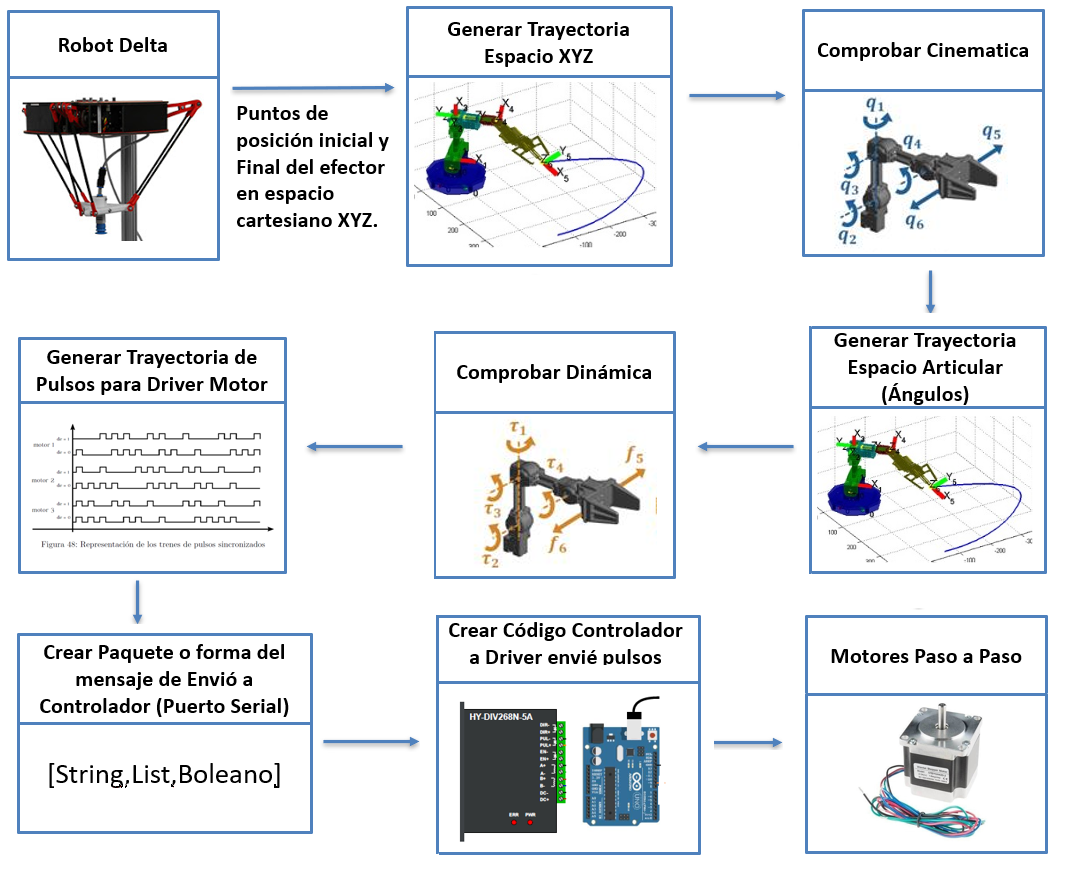
\includegraphics[width=0.8\linewidth]{Main/Chapter3/Images3/3-1/diagrama-de-flujo-robot.png}
        \caption{asd}
        \label{f:Cap3-1_diagrama_de_flujo_robot_accion}
    \end{figure}
    
Los pasos del diagrama de flujo son los siguientes:

\begin{enumerate}
    \item Definir los puntos de inicio y final de la trayectoria del robot.
    \item Elegir el tipo de trayectoria, posiciones, velocidades y aceleraciones impuestas y no dañar los componentes del robot.
    \item Comprobar la cinemática y dinámica para asegurar la trayectoria impuesta y no dañar los componentes del robot.
    \item Transformación de la trayectoria cartesiana al espacio articular de los actuadores que controlan el movimiento de las partes mecánicas del robot.
    \item Traducción de trayectoria en el espacio articular a pulsaciones que entiendan los drivers de cada motor.
    \item Envío de pulsos al driver de los motores por medio de un controlador.
\end{enumerate}

\section{Estructura de un robot delta}

    El robot delta puede ser subdivido por categorías de acuerdo al grupo estructural al que pertenezcan. Estas categorías facilitan la generación de conceptos para cada grupo de manera independiente \cite{Robot_parelelo_tipo}}
    
\section{Conexiones entre componentes}
    Desde
    
\section{Diagramas de bloques del problema}
    Desde

\section{Piezas mecánicas}
    Desde
    
    \subsection{Base fija}
        Desde
    \subsection{Brazo}
        Desde
    \subsection{Antebrazo}
        Desde
    \subsection{Efector}
        Desde
    
\section{Software Robor Operating System (ROS)}
    Desde
    \subsection{Arquitectura y conceptos}
        Desde
    \subsection{Herramientas y librerías}
        Desde

\section{Interfaz de visualización (Rviz)}
    Desde
    
\section{Software Algorithm Development and mining (ADAMS)}
Desde

    
      
        
            
            
            

        
    
    